\newcommand{\PartieI}{Partie I : L'algorithme de recommandation basé sur la factorisation matricielle}
\definecolor{darkgreen}{RGB}{0,100,0}

\begin{frame}{Sommaire}
    \begin{itemize}
        \item Introduction
        \item \textbf{L'algorithme de recommandation basé sur la factorisation matricielle}
    \end{itemize}
\end{frame}

\begin{frame}{\PartieI}
    \begin{itemize}
        \item Faisant partie du filtrage collaboratif...
        \item {
              Ce dont on dispose :
              \begin{figure}[htbp]
                  \centering
                  \hspace{80pt}
                  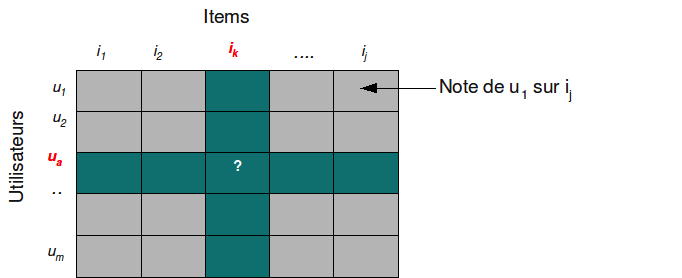
\includegraphics[width=0.6\textwidth]{ressources/matrix_users_items.png}
                  \caption{Matrice utilisateur-item notée $\mathcal{R}$}
                  \label{fig:matrix-user-item}
              \end{figure}
              }
    \end{itemize}
\end{frame}

\begin{frame}{\PartieI}
    \begin{center}
        \textcolor{red}{\textbf{\large{Problème !!}}}
    \end{center}
\end{frame}

\begin{frame}{\PartieI}
    \begin{center}
        \textcolor{darkgreen}{\textbf{\large{Solution : Factorisation Matricielle}}}
    \end{center}
\end{frame}

\begin{frame}{\PartieI}
    On note :
    \begin{itemize}
        \item $\mathcal{R}$ comme la matrice originale de taille $m \times n$, où $m$ est le nombre d'utilisateurs et $n$ est le nombre d'items.
        \item $\mathcal{P}$ comme la matrice d'utilisateurs de taille $m \times k$, où $k$ est le nombre de facteurs latents.
        \item $\mathcal{Q}$ comme la matrice d'items de taille $k \times n$.
    \end{itemize}
    \begin{center}
        \textbf{L'objectif est de trouver P et Q tels que R = PQ.}
    \end{center}
\end{frame}

\begin{frame}{\PartieI}
    L'erreur quadratique moyenne est donnée par :
    \begin{equation*}
        \min _{q, p} \sum_{(u, i) \in \kappa}\left(r_{u i}-q_i^T p_u\right)^2+\lambda\left(\left\|q_i\right\|^2+\left\|p_u\right\|^2\right)
    \end{equation*}
    où, $\kappa$ est l'ensemble des paires $(u,i)$ pour lesquels $r_{ui}$ est connue (training set).
\end{frame}

\begin{frame}{\PartieI}
    La méthode de descente de gradient stochastique (DGS) se fait avec :
    \begin{equation*}
        \begin{aligned}
             & q_i \leftarrow q_i+\gamma \cdot\left(e_{u i} \cdot p_u-\lambda \cdot q_i\right) \\
             & p_u \leftarrow p_u+\gamma \cdot\left(e_{u i} \cdot q_i-\lambda \cdot p_u\right)
        \end{aligned}
    \end{equation*}
    où $e_{u i}^{\stackrel{\text { def }}{=}} r_{u i}-q_i^T p_u$ est l'erreur de prédiction pour l'élément $r_{ui}$ de la matrice de notation.
\end{frame}

\begin{frame}{\PartieI}
    \begin{center}
        \textbf{\large{Les \textcolor{darkgreen}{avantages} et les \textcolor{red}{limites} de la méthode de descente de gradient stochastique (DGS)}}
    \end{center}
\end{frame}

\begin{frame}{\PartieI}
    \begin{center}
        \large{Une alternative : \textbf{La méthode des moindres carrés alternés (MCA)}}
    \end{center}
\end{frame}

\begin{frame}{\PartieI}
    \begin{center}
        \textbf{\large{Les \textcolor{darkgreen}{avantages} et les \textcolor{red}{limites} de la méthode des moindres carrés alternés (MCA)}}
    \end{center}
\end{frame}

\begin{frame}{\PartieI}
    \begin{center}
        \textbf{\large{Les \textcolor{darkgreen}{avantages} et les \textcolor{red}{limites} de la factorisation matricielle}}
    \end{center}
\end{frame}